
\section{recall: window size versus bandwidth}
\usetikzlibrary{arrows.meta,calc}

\begin{frame}[fragile,label=throughAndWindow]{throughput and window size}
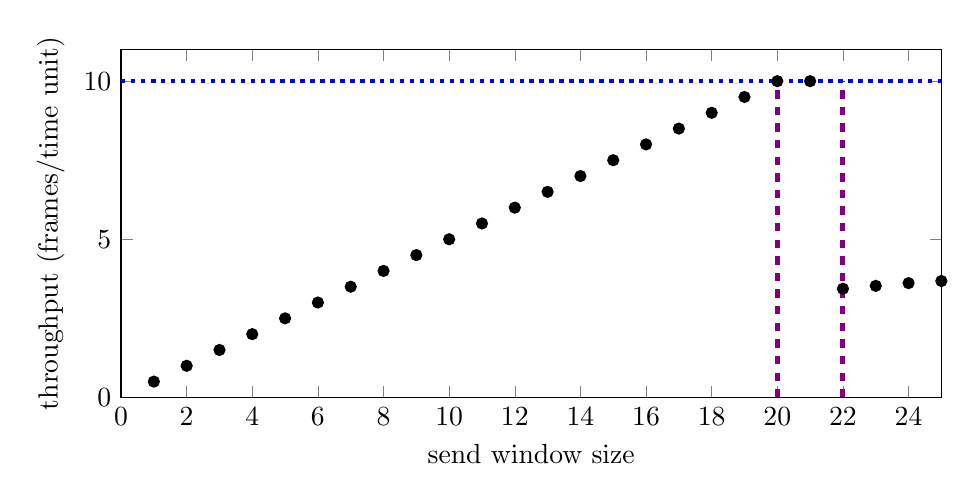
\begin{tikzpicture}
\begin{axis}[width=12cm,height=6cm,
    xlabel=send window size,
    ylabel=throughput (frames/time unit),
    xmin=0,xmax=25,ymin=0]
\addplot[only marks] coordinates {
(1, 0.5000025000125)
(2, 1.0000090000810007)
(3, 1.4999925000374998)
(4, 2.0000280003920055)
(5, 2.500037500562508)
(6, 3.000003000003)
(7, 3.5000035000035)
(8, 4.000048000576006)
(9, 4.499842505512307)
(10, 5.000025000125)
(11, 5.499975250111374)
(12, 5.99977200866367)
(13, 6.499710762871052)
(14, 6.999811005102861)
(15, 7.4996812635462975)
(16, 7.999680012799485)
(17, 8.499426288725509)
(18, 8.999361045365776)
(19, 9.499202067026369)
(20, 9.999100080971061)
(21, 9.999100080973866)
(22, 3.435635094325549)
(23, 3.5274986154570636)
(24, 3.613708966335035)
(25, 3.6808686850100703)
(26, 3.753260645186032)
(27, 3.8487443471573166)
(28, 3.925956461143474)
};
\addplot[blue,dotted,ultra thick,domain=0:25] {10};
    \draw[violet,dashed,ultra thick] (axis cs:20,0) -- (axis cs:20, 10)
     coordinate (empty queue mark);
    \draw[violet,dashed,ultra thick] (axis cs:21.99,0) -- (axis cs:21.99, 10)
     coordinate (full queue mark);
\end{axis}
\end{tikzpicture}
\end{frame}

\usetikzlibrary{arrows.meta,calc}

\begin{frame}[fragile,label=transitTime]{packet transit time}
\begin{tikzpicture}
\draw[ultra thick,arrows={-Latex}] (0, 0) node[left] {sender} -- (1, 0);
\draw[thick] (1, -.5) rectangle (3, .5);
\foreach \x in {2,2.2,2.4,2.6,2.8} {
    \draw (\x, -.5) -- (\x, .5);
}
\node[anchor=south,align=center] at (2, .5) {
    loss when full
};
\node[anchor=north,align=center] at (2, -.5) (queue label) {
    queue
};
\node[anchor=north,font=\fontsize{9}{10}\selectfont] at ([yshift=.3cm]queue label.south) {
    capacity 20
};
\draw[ultra thick,arrows={-Latex}] (3, 0) -- (12, 0) node[right]{receiver}
    node[midway,fill=white,draw=black,very thick,align=left] {
        10 data frames/time unit \\
        1 time unit delay
    }
    node[visible on=<1-3>,ultra thick,pos=0,draw=black,fill=white,font=\tiny,below=.5cm] (data-main) {data};
    \begin{visibleenv}<2->
    \draw[red,-Latex,very thick] (data-main.east) -- (data-main.west -| 13, 0) coordinate (end send)
        node[midway,below,font=\small] {1 time unit (sender to receiver)};
    \end{visibleenv}
\begin{scope}[shift={(12, -4)},x=-1cm]
    \draw[ultra thick,arrows={-Latex}] (0, 0) node[right] {receiver} -- (1, 0);
    \draw[thick] (1, -.5) rectangle (3, .5);
    \foreach \x in {2,2.2,2.4,2.6,2.8} {
        \draw (\x, -.5) -- (\x, .5);
    }
    \node[anchor=south,align=center] at (2, .5) {
        loss when full
    };
    \node[anchor=north,align=center] at (2, -.5) (queue label) {
        queue
    };
    \node[anchor=north,font=\small] at ([yshift=.2cm]queue label.south) {
        capacity 20
    };
    \draw[ultra thick,arrows={-Latex}] (3, 0) -- (12, 0) node[left]{sender}
        node[midway,fill=white,draw=black,very thick,align=left] {
            100 ACK frames/time unit \\
            1 time unit delay
        }
        node[visible on=<2->,pos=0,draw=red,fill=white,font=\tiny,below=.5cm,align=center,inner sep=0.5mm] 
            (ack-start) {a\\c\\k};
    \begin{visibleenv}<2->
        \draw[dotted,red,-Latex,very thick] (end send) |- (ack-start.east);
        \draw[red,-Latex,very thick] (ack-start.west) -- (ack-start.west -| 12, 0) node[midway,below,font=\small] { + 1 time unit (receiver to sender)};
    \end{visibleenv}
\end{scope}
\begin{visibleenv}<3>
\node[draw=red,fill=white,ultra thick,align=left] at (6, -2.5) {
    takes 1 + 1 time units to send message + receive ack \\
    goal: keep sending stuff while waiting
};
\end{visibleenv}
\end{tikzpicture}
\end{frame}

\begin{frame}{filling the pipe}
    \begin{itemize}
    \item round-trip time of 2 time units
        \begin{itemize}
        \item from send data to receive ACK (assuming no queuing delay)
        \end{itemize}
    \item can send 10 data frames per time unit
    \item = can send 20 data frames while waiting for ACK
    \vspace{.5cm}
    \item<2> \myemph{``bandwidth-delay product''}
        \begin{itemize}
        \item 10/time unit (banwidth) times 2 time unit (RTT = delay)
        \end{itemize}
    \end{itemize}
\end{frame}


\section{why optimal / counting packets in flight}
\begin{frame}{why optimal}
    \begin{itemize}
    \item in normal operation with window size $W$
        \begin{itemize}
        \item receive ACK for $x$ (now $W-1$ in flight)
        \item send packet $x+W$
        \item receive ACK for $x+1$
        \item send packet $x+W+1$
        \item \ldots
        \end{itemize}
    \item window size keeps $W$ packets in flight
    \item if links + queues can hold $W$ packets --- perfect!
    \end{itemize}
\end{frame}

\begin{frame}{number in flight on losses}
    \begin{itemize}
    \item window size $W$
    \item let's say we lose packet $x$ [only], sender might
        \begin{itemize}
        \item receive ACK for $x-1$
        \item send packet $x+W-1$
        \item receive ACK for $x$, $x$, $x$, \ldots
        \item resend packet $x$ (guess it is lost)
        \item \myemph<2>{receive ACK for $x$, $x$, $x$, \ldots}
        \item receive ACK for packet $x+W-1$ 
        \item send packets $x+W$ through $x+W+W-1$
        \end{itemize}
    \end{itemize}
\begin{tikzpicture}[overlay,remember picture]
\begin{visibleenv}<2->
\node[draw=red,ultra thick,anchor=south,align=left] at ([yshift=1cm]current page.south) {
    lots of time where we are not sending packets \\
    means network is underutilized
};
\end{visibleenv}
\end{tikzpicture}
\end{frame}

\begin{frame}{window size tweaking}
    \begin{itemize}
    \item window size imperfect proxy for \# packets in flight
    \item we'll ignore the difference for now
    \vspace{.5cm}
    \item our goal for now: window size = number of packets to have in flight
    \end{itemize}
\end{frame}



\section{searching for performance}
\usetikzlibrary{arrows.meta,shapes.misc,shapes.geometric}
\begin{frame}{finding window size empirically (1)}
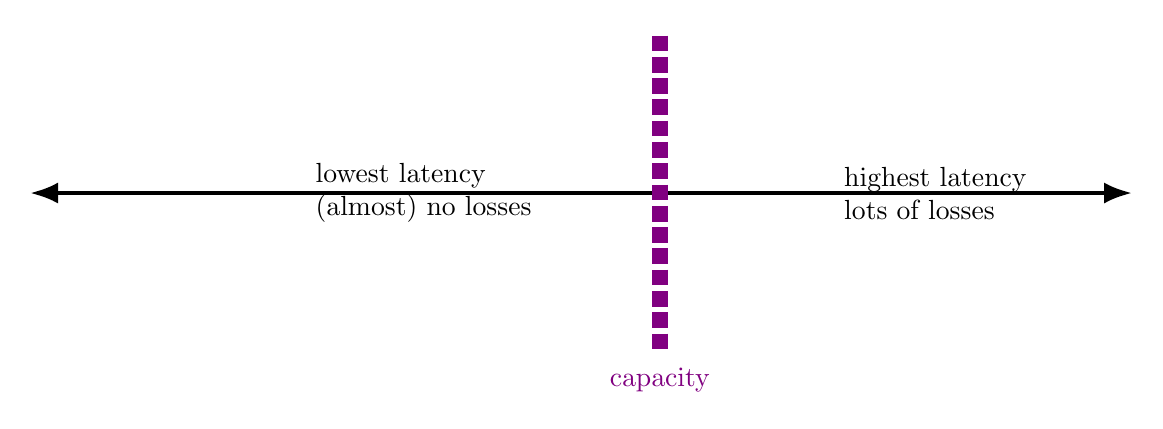
\begin{tikzpicture}
\draw[ultra thick,Latex-Latex] (-7, 0) -- (7, 0);
\draw[dotted,line width=2mm,violet] (1, 2) -- (1, -2) node[below] {capacity};
\node[align=left] at (-2, 0) {
    lowest latency \\
    (almost) no losses
};
\node[align=left] at (4.5, 0) {
    highest latency \\
    lots of losses 
};
\end{tikzpicture}
\end{frame}

\begin{frame}{key insight}
    \begin{itemize}
    \item latency/loss rate increases when window size too big
    \item latency/loss rate stable when window size not too big
    \vspace{.5cm}
    \item for now, we'll focus on loss rate
        \begin{itemize}
        \item but you can do something similar with latency
        \end{itemize}
    \end{itemize}
\end{frame}

\begin{frame}{try a bunch of things}
\begin{tikzpicture}
\tikzset{
    good/.style={draw,star,thick,fill=green!70!black},
    bad/.style={draw,cross out,red!70!black,line width=3mm},
}
\draw[ultra thick,Latex-Latex] (-7, 0) -- (7, 0);
\node at (0, -.5) {window size};
\node[good,label={east:= low loss rate}] (key good) at (-6, 2) {};
\node[bad,label={east:= high loss rate}] (key bad) at (-6, 1) {};
\begin{visibleenv}<2->
\node[good] at (-3, 0){};
\node[bad] (high bad) at (5, 0){};
\end{visibleenv}
\begin{visibleenv}<3->
\node[bad] at (1, 0){}; 
\end{visibleenv}
\begin{visibleenv}<4->
\node[good] at (-1, 0){}; 
\end{visibleenv}
\begin{visibleenv}<5->
\node[good] at (-0.5, 0){}; 
\node[good] at (-0.2, 0){}; 
\node[bad] at (0.3, 0){}; 
\node[bad] at (0.5, 0){}; 
\node[bad] at (0.9, 0){}; 
\end{visibleenv}
\begin{visibleenv}<6>
\draw[Latex-,very thick] (high bad) -- ++(-2, -5) node {
    what is the network like when we do this?
};
\end{visibleenv}
\end{tikzpicture}
\end{frame}


\section{a little history}
\begin{frame}{revisiting congestion collapse}
\includegraphics[width=0.6\textwidth]{../congest/jacobson-title}
\includegraphics[width=0.6\textwidth]{../congest/jacobson-disaster}
\end{frame}

\begin{frame}<1>[label=jacobsonFixes]{fixes from Jacobson's 1987 paper}
\begin{tikzpicture}
\node[anchor=north west] (fixes) at (0, 0) {
    \includegraphics[width=0.6\textwidth]{../congest/jacobson-fixes}
};
%\path[draw,help lines] (0, 0) grid[step=1] (8, -5);
\begin{visibleenv}<2>
    \draw[red,ultra thick] (0, -3.8) rectangle (9, -4.4);
\end{visibleenv}
\begin{visibleenv}<4>
    \draw[red,ultra thick] (0, -2) rectangle (3, -2.8);
\end{visibleenv}
\begin{visibleenv}<3>
    \draw[red,ultra thick] (0, -5.4) rectangle (4.5, -6.2);
\end{visibleenv}
\end{tikzpicture}
\end{frame}


\section{changing cross-traffic}

\usetikzlibrary{arrows.meta,calc,shapes}
\providecommand{\computer}{%
    \includegraphics[width=1cm]{../common/Noun_project_216.pdf}
}
\providecommand{\switch}{%
    \includegraphics[width=0.9cm]{../common/fig-switch.pdf}
}
\providecommand{\router}{%
    \includegraphics[width=0.9cm]{../common/fig-router.pdf}
}



\begin{frame}{changing cross-traffic}
\begin{tikzpicture}
\tikzset{
    computer/.style={inner sep=0mm,outer sep=0mm,execute at begin node={\computer}},
    switch/.style={inner sep=0mm,outer sep=0mm,execute at begin node={\switch}},
    router/.style={inner sep=0mm,outer sep=0mm,execute at begin node={\router},circle},
    connect/.style={draw,very thick,Latex-Latex},
    connect big/.style={draw,ultra thick,Latex-Latex},
}
\node[computer] (A) at (0, 0){};
\node[computer] (B) at (13, 0){};
\node[router] (r1) at (5, 0){};
\node[router] (r2) at (10, 0){};
\node[computer] (C) at (3, 3){};
\node[computer] (D) at (12, -3){};
\foreach \x/\y in {A/r1,r1/r2,r2/B,C/r1,r2/D} {
    \draw[connect] (\x) -- (\y);
}
\begin{visibleenv}<2>
\foreach \x/\y in {A/r1,r1/r2,r2/B} {
    \draw[blue,line width=1mm] ([yshift=-1mm]\x) -- ([yshift=-1mm]\y);
}
\node[text=blue,anchor=north] at ([yshift=-3mm]$(A)!0.5!(r1)$) {10Mbit};
\end{visibleenv}
\begin{visibleenv}<3>
\foreach \x/\y in {A.east/r1.west,r1.east/r2.west,r2.east/B.west} {
    \draw[-Latex,blue,line width=1mm] ([yshift=-3mm]\x) -- ([yshift=-3mm]\y);
}
\foreach \x/\y in {C/r1,r1.east/r2.west,r2/D} {
    \draw[-Latex,red,dotted,line width=1mm] ([yshift=3mm]\x) -- ([yshift=3mm]\y);
}
\node[text=blue,anchor=north] at ([yshift=-3mm]$(A)!0.5!(r1)$) {\sout{10Mbit} 7Mbit};
\node[text=red,anchor=west] at ($(C)!0.5!(r1)$) {3Mbit};
\end{visibleenv}
\begin{visibleenv}<4>
\foreach \x/\y in {A/r1,r1/r2,r2/B} {
    \draw[blue,line width=1mm] ([yshift=-1mm]\x) -- ([yshift=-1mm]\y);
}
\node[text=blue,anchor=north] at ([yshift=-3mm]$(A)!0.5!(r1)$) {\sout{10Mbit} \sout{7Mbit} 10Mbit};
\end{visibleenv}
\end{tikzpicture}
\end{frame}

\begin{frame}{adapting to cross-traffic}
    \begin{itemize}
    \item available bandwidth will change
    \item previous example: 3Mbit lost/added from other flow
    \vspace{.5cm}
    \item need to adapt to lost bandwidth
    \item need to detect new available bandwidth
    \end{itemize}
\end{frame}

\begin{frame}{other flow's bandwidth?}
    \begin{itemize}
    \item for now, we'll pretend other flows don't react to us
    \vspace{.5cm}
    \item later topic: what happens when both reacting?
    \end{itemize}
\end{frame}


\section{part 1: window sizing}
\againframe<2>{jacobsonFixes}

\section{focus on steady state}
\begin{frame}{handling steady state}
    \begin{itemize}
    \item most of the time we should be at approx. correct window size
    \vspace{.5cm}
    \item want to focus on how we react to changes
    \item still going to use ``experimentation'' idea
    \end{itemize}
\end{frame}


\section{up/down pattern (rough)}
\begin{frame}{window size experimenting}
\begin{itemize}
\item increase window size until see losses
    \begin{itemize}
    \item note: need at least one round-trip-time to see effect of new window
    \end{itemize}
\item decrease window size on losses
\end{itemize}
\end{frame}

    % FIXME: show sawtooth pattern

\section{performance collapse}
\begin{frame}{the overloaded switch}
\begin{itemize}
\item let's say switch can handle 50 packets/second
\item but has:
    \begin{itemize}
    \item 100 packets/second from test flow sending as fast as it can
    \item 10 packets/second from other session
    \end{itemize}
\item expected \textit{loss rate} (\% packets lost)?
\item expected \% test flow packets lost?
\item expected other session packets lost?
\end{itemize}
\end{frame}

\begin{frame}{modeling who gets dropped}
    \begin{itemize}
    \item it kinda does matter\ldots
    \item sending in big bursts or spread out (``pacing'')?
        \begin{itemize}
        \item bursts can overload queues even though average rate is low
        \end{itemize}
    \item how switch's queue works?
        \begin{itemize}
        \item queue size (handling bursts), way to choose what to drop
        \end{itemize}
    \item random or fixed intervals between sending?
    \vspace{.5cm}
    \item<2-> but we'll \myemph<2>{simplify}, assuming---
        \begin{itemize}
        \item a flow's arrivals are randomly spaced
        \item drops hit packets at random
        \item queue is ``pretty big''
        \end{itemize}
    \end{itemize}
\end{frame}

\begin{frame}{the overloaded switch}
\begin{itemize}
\item let's say switch can handle 50 packets/second
\item but has:
    \begin{itemize}
    \item 100 packets/second from test flow (checking window size) 
    \item 20 packets/second from other session
    \end{itemize}
\item expected \textit{loss rate} (\% packets lost)? $\frac{100+20-50}{100+20}=58\%$
\item expected \% test flow packets lost? $58\%$
\item expected \% other session packets lost? $58\%$
\item<2-> \myemph{\ldots but I missed something}
\end{itemize}
\end{frame}

\begin{frame}{a virtuous cycle}
\begin{itemize}
\item what is other session going to when 58\% of its packets are lost?
    \begin{itemize}
    \item probably resend them
    \end{itemize}
\item what about when resent packets are lost?
    \begin{itemize}
    \item probably resent again
    \end{itemize}
\vspace{.5cm}
\item if other session doesn't slow down, then\ldots
\item $10$ pkt/s $\rightarrow10+58\%\cdot10+58\%^2\cdot10 \ldots\approx 48$ pkt/s
\end{itemize}
\end{frame}


\begin{frame}{the overloaded switch (revised)}
\begin{itemize}
\item let's say switch can handle 50 packets/second
\item but has:
    \begin{itemize}
    \item 100 packets/second from test flow (checking window size) 
    \item 20 packets/second from other session $\rightarrow 48$ with resends
    \end{itemize}
\item expected \textit{loss rate} (\% packets lost)? $\frac{100+48-50}{100+48}=66\%$
\item expected \% test flow packets lost? $66\%$
\item expected \% other session packets lost? $66\%$
    \begin{itemize}
    \item<2-> means that 48 pkt/sec is slight underestimate
    \item<2-> though realistically other session should slow down
    \end{itemize}
\end{itemize}
\end{frame}

\begin{frame}{aside: latency (1)}
\begin{itemize}
\item 58\% packet loss $\rightarrow$ average packet sent 2.4 times
\item need one round-trip time (RTT) to detect loss
    \begin{itemize}
    \item probably from duplicate ACK
    \item if detecting via timeout, probably longer
    \end{itemize}
\item so need 1.4 RTTs (detecting loss 1.4 times) extra time 
\item mean latency $= \frac{1.4 \text{RTTs}}{0.5 \text{RTTs}}$ times normal $= 2.8$ times normal
\end{itemize}
\end{frame}

\begin{frame}{aside: high-percentile latency}
\begin{itemize}
\item 58\% packet loss
\item about 10\% of time need more than 4 retransmissions
\item about 5\% of the time need more than 5 retransmissions
\item about 1\% of the time need more than 8 retransmissions
\end{itemize}
\end{frame}

\begin{frame}{sliding windows and retransmissions}
    \begin{itemize}
    \item assuming that other session doesn't slow down
    \vspace{.5cm}
    \item sliding window approach slows down on losses
    \end{itemize}
\end{frame}

\begin{frame}{sliding window throughput collapse}
\begin{itemize}
\item let's say doing sliding window with 100 packet window
\item if 1\% of the time, we need to resend a packet 8 times, then
\item probably need around 8 RTTs to send all 100 packets in window
\vspace{.5cm}
\item<2-> $\approx$ 8 times slower with same window size
\end{itemize}
\end{frame}

\begin{frame}{performance v load}
\begin{tikzpicture}

\end{tikzpicture}
\end{frame}


\section{heuristic: slow increase}
\begin{frame}{slow increase}
    \begin{itemize}
    \item want to increase \textit{slowly} to avoid overload
    \item original TCP: +1 packet/round trip time
    \vspace{.5cm}
    \item<2-> +1 certainly not optimal choice, but okay heuristic
    \item<2-> important theoretically: approx. \myemph{additive} increase
        \begin{itemize}
        \item helps ensure good behavior with multiple connections
        \item (we'll talk later about why)
        \end{itemize}
    \end{itemize}
\end{frame}


\subsection{exercise: convergence times}
\begin{frame}{exercise: convergence time (1)}
    \begin{itemize}
    \item suppose: 50 ms round trip time
    \item initially sending at 600 packets/second
        \begin{itemize}
        \item $\approx 0.9$Mbyte/sec with 1500 byte packets
        \end{itemize}
    \item optimal rate is 10000 packets/second
        \begin{itemize}
        \item $\approx 15$Mbyte/sec with 1500 byte packets
        \end{itemize}
    \item how long to get there?
    \vspace{.5cm}
    \item<2-> current: 30 packets/RTT (= window size 30)
    \item<2-> need to get to: 500 packets/RTT
    \item<2-> will take $500-30=470$ round trips $\approx$ 23500 ms $\approx$ 24 s
    \end{itemize}
\end{frame}


\section{heuristic: fast decrease}
\begin{frame}{fast decrease (v2)}
    \begin{itemize}
    \item resetting window size to 1 is too slow
    \item compromise:
        \begin{itemize}
        \item loss detected without timeout: divide window size by two
        \item loss detected with timeout: decrease to 1
        \end{itemize}
    \vspace{.5cm}
    \item<2-> exactly by two probably not important
    \item<2-> important theoretically: \myemph{multiplicative} decrease
        \begin{itemize}
        \item will help show okay behavior with multiple flows
        \end{itemize}
    \end{itemize}
\end{frame}



    % FIXME: hilite distance measurement oof down parts on sawtooth pattern

\section{some graphs}
\begin{frame}[label=vegasrenotrace]{}
\includegraphics[width=0.9\textwidth]{../congest/vegas-fig1} \\
{
    \tiny from Brakmo, O'Malley, and Peterson, ``TCP Vegas: New techniques for
congestion detection and avoidance''} \\
    \small top thick, light-grey line = congestion window; dotted = slow start threshold
\end{frame}




\section{`slow start'}
\againframe<4>{jacobsonFixes}

\begin{frame}{``slow start''}
    \begin{itemize}
    \item not very well named
    \vspace{.5cm}
    \item exponential(ish) increase to find window size 
        \begin{itemize}
        \item used on connection setup or some losses
        \end{itemize}
    \vspace{.5cm}
    \item history: original TCP set high window size
    \item slow start is ``slow'' because it starts at a small size always
    \item \ldots but it grows \myemph{really quickly}
    \end{itemize}
\end{frame}

\begin{frame}{``slow start''}
    \begin{itemize}
    \item set window size = 1 packet
    \item increase by one packet for each ACK
    \item \ldots until first packet loss
    \item use window size before first window size
    \end{itemize}
\end{frame}

 % FIXME: picture

\subsection{exercise}
\begin{frame}{slow start effect}
    \begin{itemize}
    \item suppose we never leave slow start in connection between A and B and:
    \vspace{.5cm}
    \item A sends 4 packets to B
    \item after receiving 4 packets, B sends 8 packets to A
    \item after receiving those packets A sends 1 packet to B
    \vspace{.5cm}
    \item how many round-trip times does this take?
    \end{itemize}
\end{frame}


\subsection{some more graphs}
\againframe<2>{vegasrenotrace}
\begin{frame}{TCP `Tahoe' w/ one loss}
\tiny from Kevin Fall and Sally Floyd, ``Simulation-based Comparisons of Tahoe, Reno, and SACK TCP'' \\
\includegraphics[width=\textwidth]{../congest/fall-floyd-fig2-tahoe} \\
TCP Tahoe = slow start, fast retransmit, no fast recovery 
\end{frame}

\begin{frame}{TCP `Reno' w/ one loss}
\tiny from Kevin Fall and Sally Floyd, ``Simulation-based Comparisons of Tahoe, Reno, and SACK TCP'' \\
\includegraphics[width=\textwidth]{../congest/fall-floyd-fig2-reno}
TCP Reno = slow start, fast retransmit/recovery
\end{frame}


\subsection{exercise: non-congestion losses}
\begin{frame}{non-congestion losses}
    \begin{itemize}
    \item we were ignoring non-congestion losses
    \item suppose \myemph{1\%} loss rate from transmission errors
    \item if huge bandwidth, 50 ms RTT
    \item with TCP heuristics (+1 packet/RTT, half on loss)\ldots
    \item normal window size? achieved bandwidth (pkts/sec)?
        \begin{itemize}
        \item<2-> window size increases for about 100 packets, then halves
        \item<2-> starting at window size 8:
        \item<2-> 8, 9 (17 total), 10 (27), 11 (38), 12 (50), 13 (63), 14 (77), 15 (92), 16 (>100)
        \item<2-> $\rightarrow$ window size fluctuates from around 8 to 16
        \item<3-> 12 pkts/50 ms = 240 pkts/sec
        \end{itemize}
    \end{itemize}
\end{frame}

\begin{frame}{non-congestion losses and congestion control}
    \begin{itemize}
    \item significant non-congestion losses $\rightarrow$ very bad performance with most congestion control
    \item reason why wireless, etc. often does its own acknowledgements and resending
    \end{itemize}
\end{frame}



% FIXME: \subsection{exercise: convergence times}


